\documentclass[a4paper,14pt]{extarticle}

\usepackage[utf8x]{inputenc}
\usepackage[T1]{fontenc}
\usepackage[russian]{babel}
\usepackage{hyperref}
\usepackage{indentfirst}
\usepackage{here}
\usepackage{array}
\usepackage{graphicx}
\usepackage{caption}
\usepackage{subcaption}
\usepackage{chngcntr}
\usepackage{amsmath}
\usepackage{amssymb}
\usepackage[left=2cm,right=2cm,top=2cm,bottom=2cm,bindingoffset=0cm]{geometry}
\usepackage{multicol}
\usepackage{multirow}
\usepackage{titlesec}
\usepackage{listings}
\usepackage{color}
\usepackage{enumitem}
\usepackage{cmap}
\usepackage{url}

\definecolor{green}{rgb}{0,0.6,0}
\definecolor{gray}{rgb}{0.5,0.5,0.5}
\definecolor{purple}{rgb}{0.58,0,0.82}

\lstdefinelanguage{none}{}

\lstset{
	language={Python},
	backgroundcolor=\color{white},
	commentstyle=\color{green},
	keywordstyle=\color{blue},
	numberstyle=\color{gray}\scriptsize\ttfamily,
	stringstyle=\color{purple},
	basicstyle=\lst@ifdisplaystyle\footnotesize\fi\ttfamily,
	breakatwhitespace=false,
	breaklines=true,
	captionpos=b,
	keepspaces=true,
	numbers=left,
	numbersep=5pt,
	showspaces=false,
	showstringspaces=false,
	showtabs=false,
	tabsize=4,
	frame=single,
	morekeywords={},
	deletekeywords={},
	extendedchars=false,
	columns=fullflexible,
	literate=%
		{~}{{\raise.25ex\hbox{$\mathtt{\sim}$}}}{1}%
		{-}{-}{1}
}

\titleformat*{\section}{\large\bfseries}
\titleformat*{\subsection}{\normalsize\bfseries}
\titleformat*{\subsubsection}{\normalsize\bfseries}
\titleformat*{\paragraph}{\normalsize\bfseries}
\titleformat*{\subparagraph}{\normalsize\bfseries}

\counterwithin{figure}{section}
\counterwithin{equation}{section}
\counterwithin{table}{section}
\newcommand{\sign}[1][5cm]{\makebox[#1]{\hrulefill}}
\newcommand{\equipollence}{\quad\Leftrightarrow\quad}
\newcommand{\no}[1]{\overline{#1}}
\newcommand{\code}[1]{\lstinline[language=none]|#1|}
\graphicspath{{../pics/}}
\captionsetup{justification=centering,margin=1cm}
\def\arraystretch{1.3}
\setlength\parindent{5ex}
\titlelabel{\thetitle.\quad}

\setitemize{topsep=0em, itemsep=0em}
\setenumerate{topsep=0em, itemsep=0em}


\begin{document}

\begin{titlepage}
\begin{center}
	Санкт-Петербургский Политехнический Университет Петра Великого\\[0.3cm]
	Институт компьютерных наук и технологий \\[0.3cm]
	Кафедра компьютерных систем и программных технологий\\[4cm]

	\textbf{ОТЧЕТ}\\
	\textbf{по лабораторной работе}\\[0.5cm]
	\textbf{<<Поиск векторов смещения>>}\\[0.1cm]
	Разработка графических приложений\\[3.0cm]
\end{center}

\begin{flushright}
	\begin{minipage}{0.5\textwidth}
		\textbf{Работу выполнил студент}\\[3mm]
		гр. 3540901/91502 \hfill \sign[1.1cm] \hfill Дьячков В.В.\\[5mm]
		\textbf{Работу принял преподаватель}\\[5mm]
		\sign[5cm] \hfill Абрамов Н.А. \\[5mm]
	\end{minipage}
\end{flushright}

\vfill

\begin{center}
	Санкт-Петербург\\[0.3cm]
	\the\year
\end{center}
\end{titlepage}

\addtocounter{page}{1}


\tableofcontents
\newpage

\section{Программа работы}

Реализовать алгоритмы выделения границ объектов с использованием:

\begin{enumerate}
	\item оператора Робертса;
	\item оператора Собеля;
	\item оператора Прюитта.
\end{enumerate}

\section{Выполнение работы}

\subsection{Операция свертки}

Свертка является общим методом обработки изображений, изменяющим интенсивность пикселя для отражения интенсивности окружающих пикселей. Используя свертку, можно получить различные эффекты изображений, в том числе и обнаружение границ. Главным элементом свертки является ядро свертки -- матрица (чаще всего используется квадратная матрица).

При вычислении нового значения выбранного пикселя изображения, ядро свертки накладывается своим центром на этот пиксель. Соседние пиксели так же накрываются ядром. Затем вычисляется сумма произведений значений пикселей изображения на значения, накрывшего данный пиксель элемента ядра. Полученная сумма и является новым значением выбранного пикселя. На рис. \ref{fig:convolution} приведен пример применения ядра к одному из пикселей изображения.

\begin{figure}[H]
	\centering
	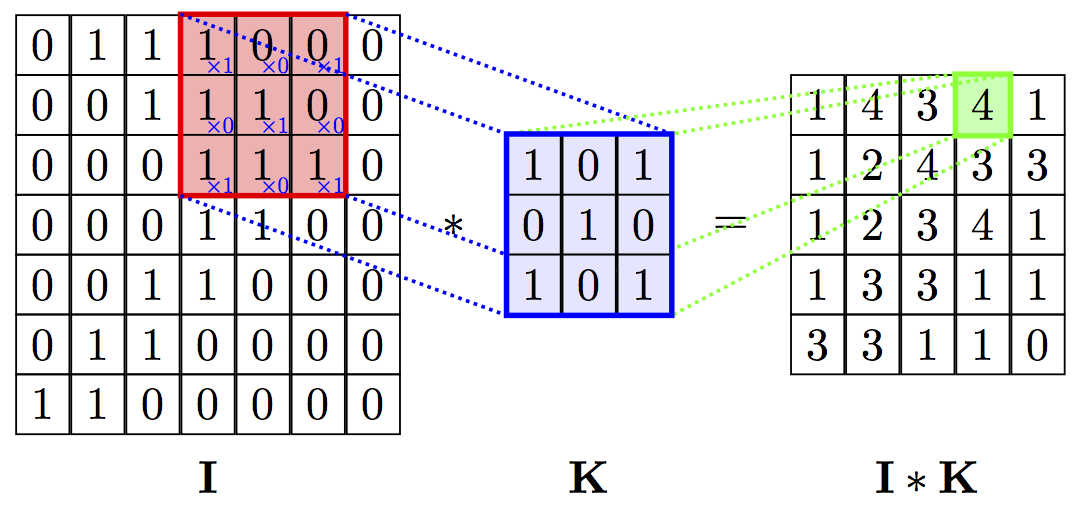
\includegraphics[width=0.8\linewidth]{convolution}
	\caption{Применение свертки к изображению}
	\label{fig:convolution}
\end{figure}

\newpage

Реализуем операцию свертки при помощи языка Python.

\begin{lstlisting}
def apply_kernel(img, kernel):
    K = kernel.shape[0]
    height = img.shape[0] - (K // 2) * 2
    width = img.shape[1] - (K // 2) * 2
    res = np.zeros((height, width))
    for i in np.arange(height):
        for j in np.arange(width):
            m = img[i:i+K, j:j+K] * kernel
            res[i][j] = m.sum()
    return np.clip(res, 0, 255).astype(np.uint8)
\end{lstlisting}

Убедимся, что разработанная функция свертки изображения работает верно, сравнив результат с функцией \code{cv.filter2D}, находящейся в библиотеке OpenCV. Для этого подадим функциям на вход одно и то же изображение и ядро. Дополнительно измерим время работы функций при помощи magic-команды Jupyter -- \code{\%\%timeit}. Строки, начинающиеся с \code{##} обозначают вывод команды.

\begin{lstlisting}
kernel = np.array([[1, 0], [0, -1]])
spb_apply_kernel = apply_kernel(spb, kernel)
spb_cv_filtered = cv.filter2D(spb, -1, kernel)
np.all(spb_cv_filtered[1:-1, 1:-1] == spb_apply_kernel)
## True

%%timeit
apply_kernel(spb, kernel)
## 1.83 s ± 71.8 ms per loop (mean ± std. dev. of 7 runs, 1 loop each)

%%timeit
cv.filter2D(spb, -1, kernel)
## 154 µs ± 6.07 µs per loop (mean ± std. dev. of 7 runs, 10000 loops each)
\end{lstlisting}

Видно, что результаты работы функций идентичны, с точностью до рамок изображения. Дело в том, что разработанная функция возвращает изображение, меньшее, чем оригинальное, на $2 * (K // 2)$ пикселей ($K$ -- размер ядра, $//$ -- целочисленное деление). Библиотечная функция \code{cv.filter2D} возвращает изображение с таким же размером, что и входное.

Время работы библиотечной функции оказалось на несколько порядков меньше. Скорее всего, это связано с ее более эффективной реализацией внутри библиотеки (например, при помощи распараллеливания применения свертки). В дальнейшем будем использовать библиотечную реализацию свертки.

\newpage

\subsection{Оператор Робертса}

Перекрестный оператор Робертса (Roberts) -- один из ранних алгоритмов выделения границ, который вычисляет на плоском дискретном изображении сумму квадратов разниц между диагонально смежными пикселами. Это может быть выполнено сверткой изображения с двумя ядрами:
$$
h_1 = \begin{bmatrix} 1 & 0 \\ 0 & -1 \end{bmatrix},\ 
h_2 = \begin{bmatrix} 0 & 1 \\ -1 & 0 \end{bmatrix}
$$

Итоговая величина перепада $G$ получемого изображения получается по одной из формул:
\begin{align*}
G &= \sqrt{(h_1 * I) ^ 2 + (h_2 * I) ^ 2}\\
  &= \left| h_1 * I \right| + \left| h_2 * I \right|,
\end{align*}
где $I$ -- исходное изображение, а $*$ -- операция свертки. Первая формула использует Евклидову метрику, а вторая -- манхэттенскую.

Реализуем функцию для применения оператора Робертса. Будем использовать манхэттенскую метрику для комбинации получаемых после сверток изображений.

\begin{lstlisting}[caption={Фунукция для применения оператора Робертса}]
h1 = np.array([
    [1, 0],
    [0, -1]
])
h2 = np.array([
    [0, 1],
    [-1, 0]
])
def roberts(img):
    img_h1 = cv.filter2D(img, -1, h1)
    img_h2 = cv.filter2D(img, -1, h2)
    img_roberts = np.abs(img_h1) + np.abs(img_h2)
    return img_roberts, img_h1, img_h2
\end{lstlisting}

Применим оператор Робертса к нескольким изображениям.

\begin{figure}[H]
	\centering
	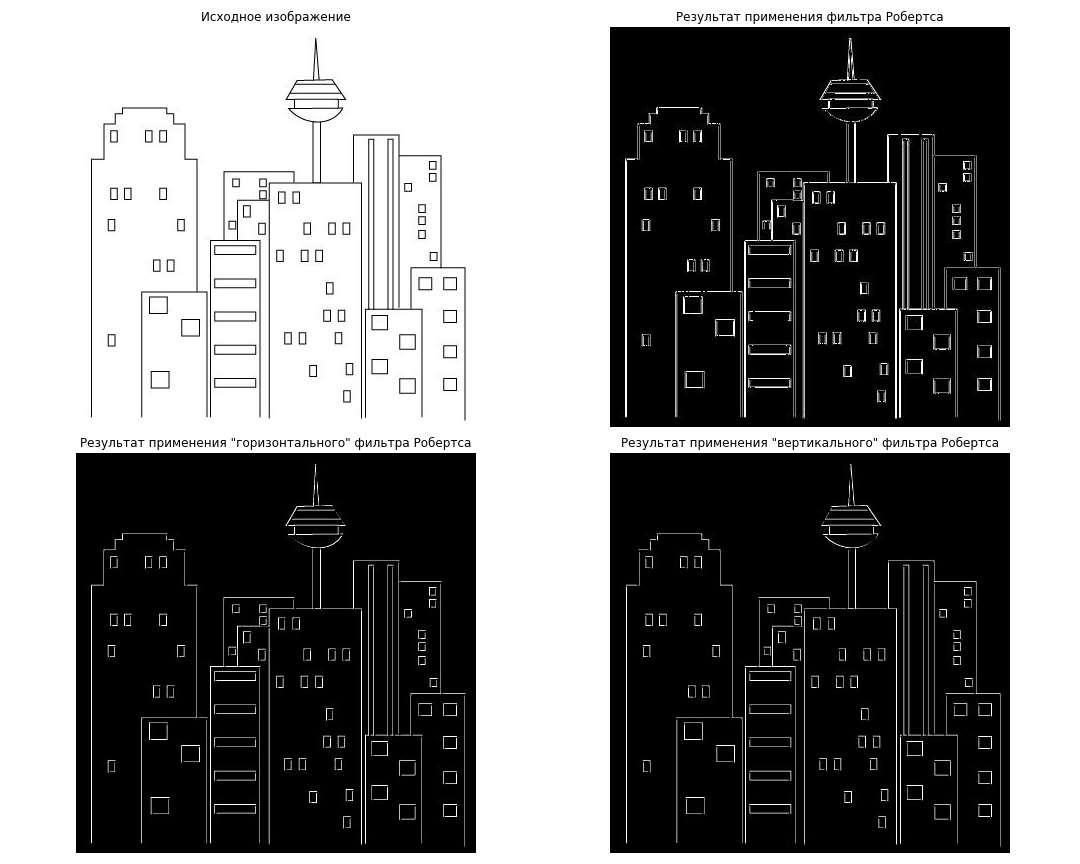
\includegraphics[width=\linewidth]{city_roberts}
	\caption{Применение оператора Робертса (1)}
\end{figure}

\begin{figure}[H]
	\centering
	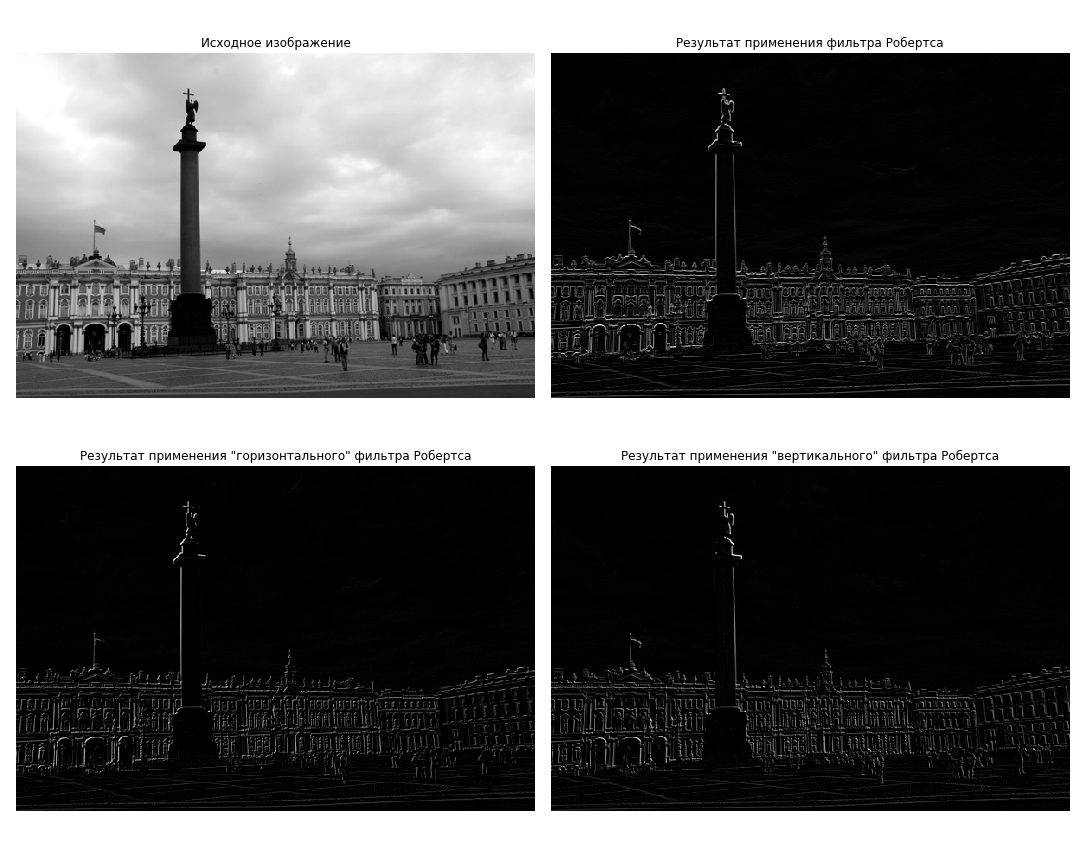
\includegraphics[width=\linewidth]{spb_roberts}
	\caption{Применение оператора Робертса (2)}
\end{figure}

\begin{figure}[H]
	\centering
	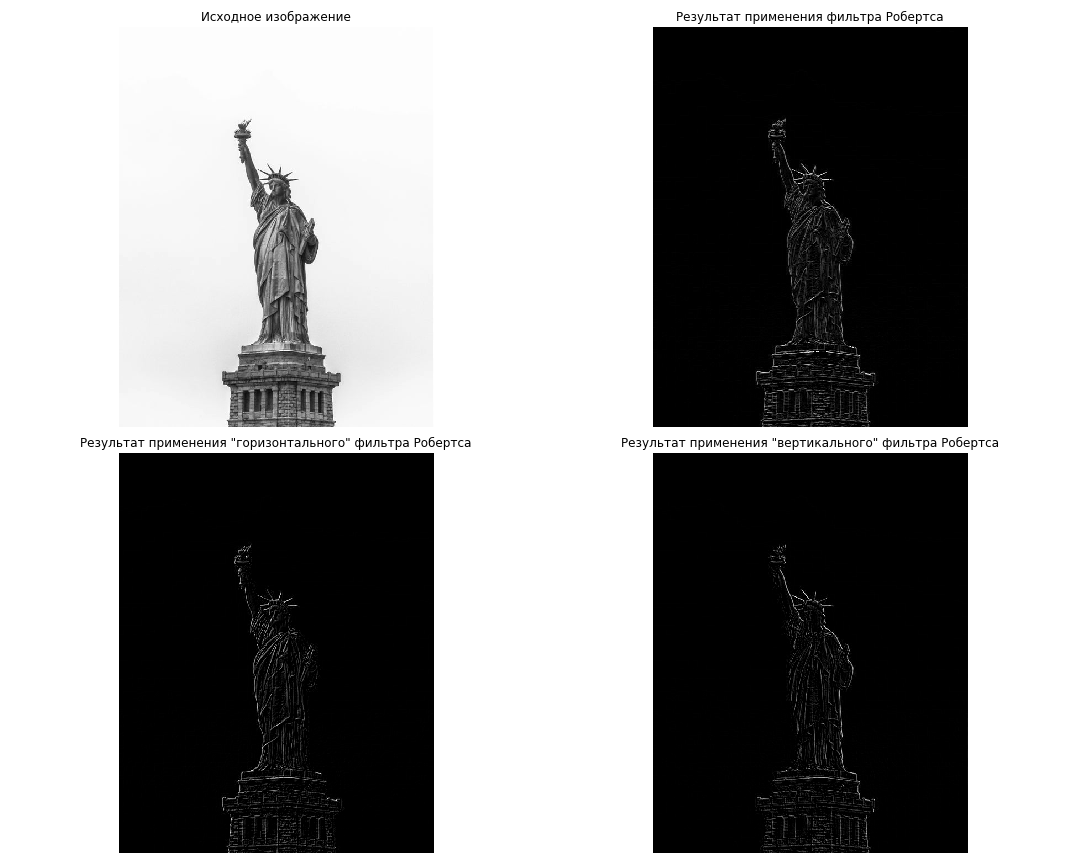
\includegraphics[width=\linewidth]{ny_roberts}
	\caption{Применение оператора Робертса (3)}
\end{figure}

\newpage

\subsection{Оператор Собеля}

Применим другой оператор для детектирования границ -- оператор Собеля (Sobel). Он основан на свертке изображения небольшими сепарабельными целочисленными фильтрами в вертикальном и горизонтальном направлениях, поэтому его относительно легко вычислять. С другой стороны, используемая им аппроксимация градиента достаточно грубая, особенно это сказывается на высокочастотных колебаниях изображения.

Оператор вычисляет градиент яркости изображения в каждой точке. Так находится направление наибольшего увеличения яркости и величина ее изменения в этом направлении. Результат показывает, насколько <<резко>> или <<плавно>> меняется яркость изображения в каждой точке, а значит, вероятность нахождения точки на грани, а также ориентацию границы.

Оператор использует ядра $3 \times 3$, с которыми сворачивается исходное изображение для вычисления приближенных значений производных по горизонтали и по вертикали.
$$
x = \begin{bmatrix}
-1 & 0 & 1 \\
-2 & 0 & 2 \\
-1 & 0 & 1
\end{bmatrix},\ 
y = \begin{bmatrix}
-1 & -2 & -1 \\
0  & 0  & 0 \\
1  & 2  & 1
\end{bmatrix} = x^T
$$

В каждой точке изображения приближенное значение величины и направления градиента можно вычислить путем использования полученных приближенных значений производных:
$$
Edge Magnitude = \sqrt{x^2 + y^2},\ Edge Direction = \tan^{-1}\frac{y}{x}
$$

Реализуем функцию для применения оператора Собеля.

\begin{lstlisting}[caption={Применение оператора Собеля}]
sx = np.array([
    [-1, 0, 1],
    [-2, 0, 2],
    [-1, 0, 1]
])
sy = sx.T
def sobel(img):
    img_x = cv.filter2D(img, -1, sx).astype(np.single)
    img_y = cv.filter2D(img, -1, sy).astype(np.single)
    img_sobel = np.sqrt(img_x ** 2 + img_y ** 2)
    return img_sobel, img_x, img_y
\end{lstlisting}

Применим оператор Собеля к нескольким изображениям.

\begin{figure}[H]
	\centering
	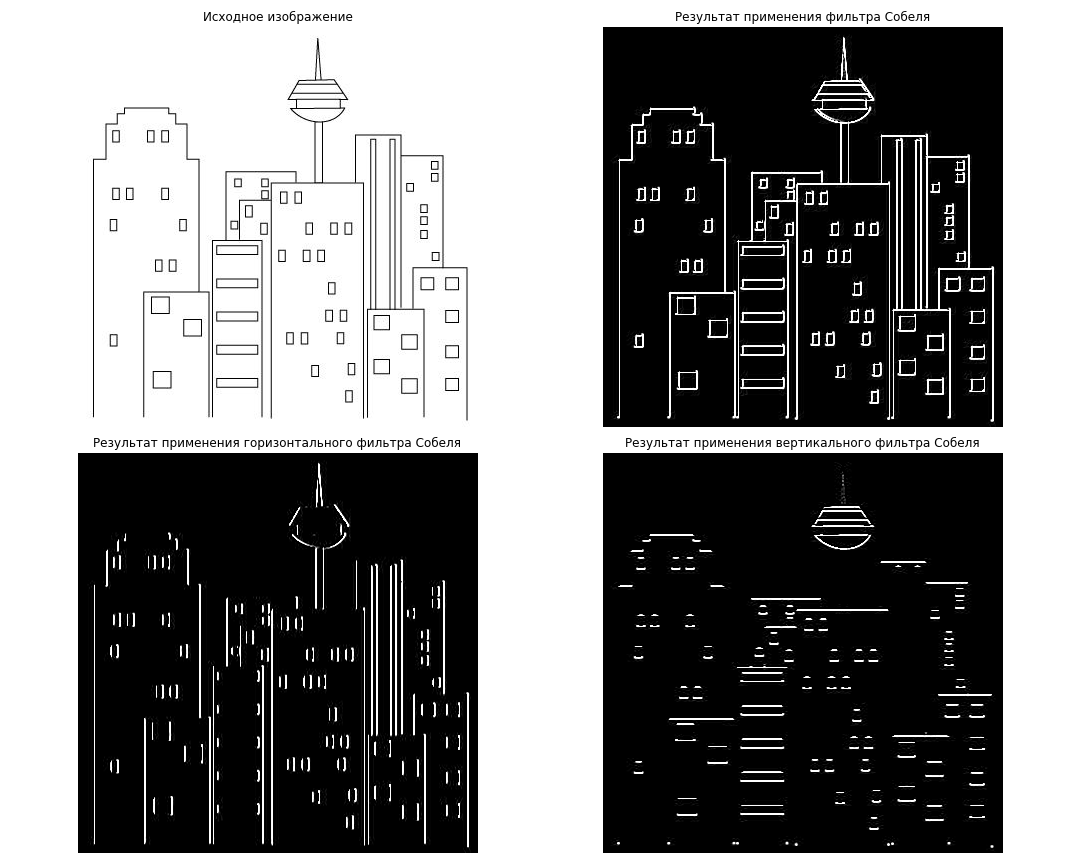
\includegraphics[width=\linewidth]{city_sobel}
	\caption{Применение оператора Собеля (1)}
\end{figure}

\begin{figure}[H]
	\centering
	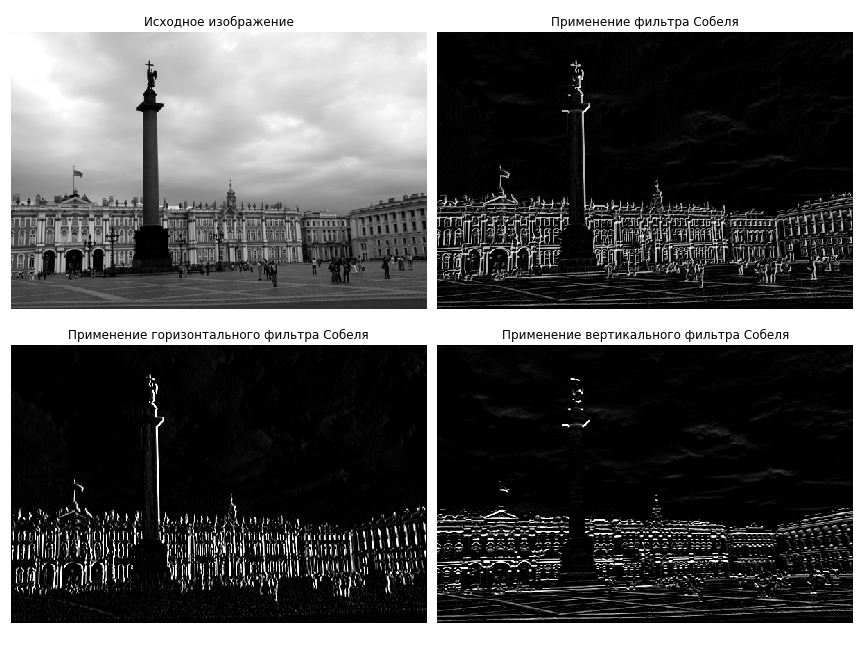
\includegraphics[width=\linewidth]{spb_sobel}
	\caption{Применение оператора Собеля (2)}
\end{figure}

\begin{figure}[H]
	\centering
	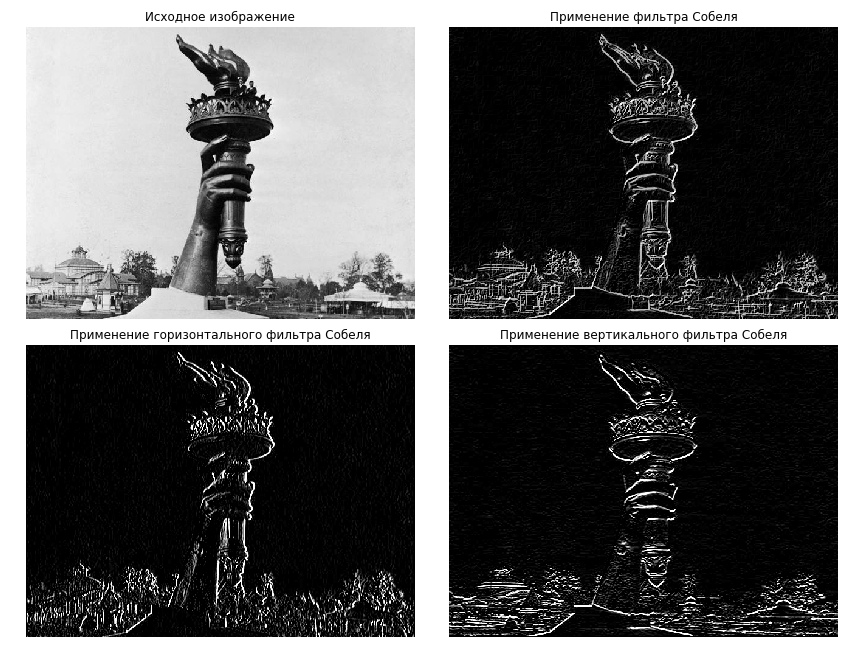
\includegraphics[width=\linewidth]{ny_sobel}
	\caption{Применение оператора Собеля (3)}
\end{figure}

\newpage

\subsection{Оператор Прюитта}

Воспользуемся еще одним оператором для детектирования границ -- оператором Прюитта (Prewitt). Этод метод вычисляет максимальный отклик на ядрах свертки для нахождения локальной ориентации границы в каждом пикселе. Этот оператор совпадает с оператором Собеля, но использует другие ядра:
$$
x = \begin{bmatrix}
-1 & 0 & 1 \\
-1 & 0 & 1 \\
-1 & 0 & 1
\end{bmatrix},\ 
y = \begin{bmatrix}
-1 & -1 & -1 \\
0  & 0  & 0 \\
1  & 1  & 1
\end{bmatrix} = x^T
$$

Оператор вычисляет градиент яркости изображения в каждой точке. Так находится направление наибольшего увеличения яркости и величина ее изменения в этом направлении. Результат показывает, насколько <<резко>> или <<плавно>> меняется яркость изображения в каждой точке, а значит, вероятность нахождения точки на грани, а также ориентацию границы.

Реализуем функцию для применения оператора Прюитта.

\begin{lstlisting}[caption={Применение оператора Собеля}]
px = np.array([
    [-1, 0, 1],
    [-1, 0, 1],
    [-1, 0, 1]]
)
py = px.T
def prewitt(img):
    img_x = cv.filter2D(img, -1, px).astype(np.single)
    img_y = cv.filter2D(img, -1, py).astype(np.single)
    img_prewitt = np.sqrt(img_x ** 2 + img_y ** 2)
    return img_prewitt, img_x, img_y
\end{lstlisting}

Применим оператор Прюитта к нескольким изображениям.

\begin{figure}[H]
	\centering
	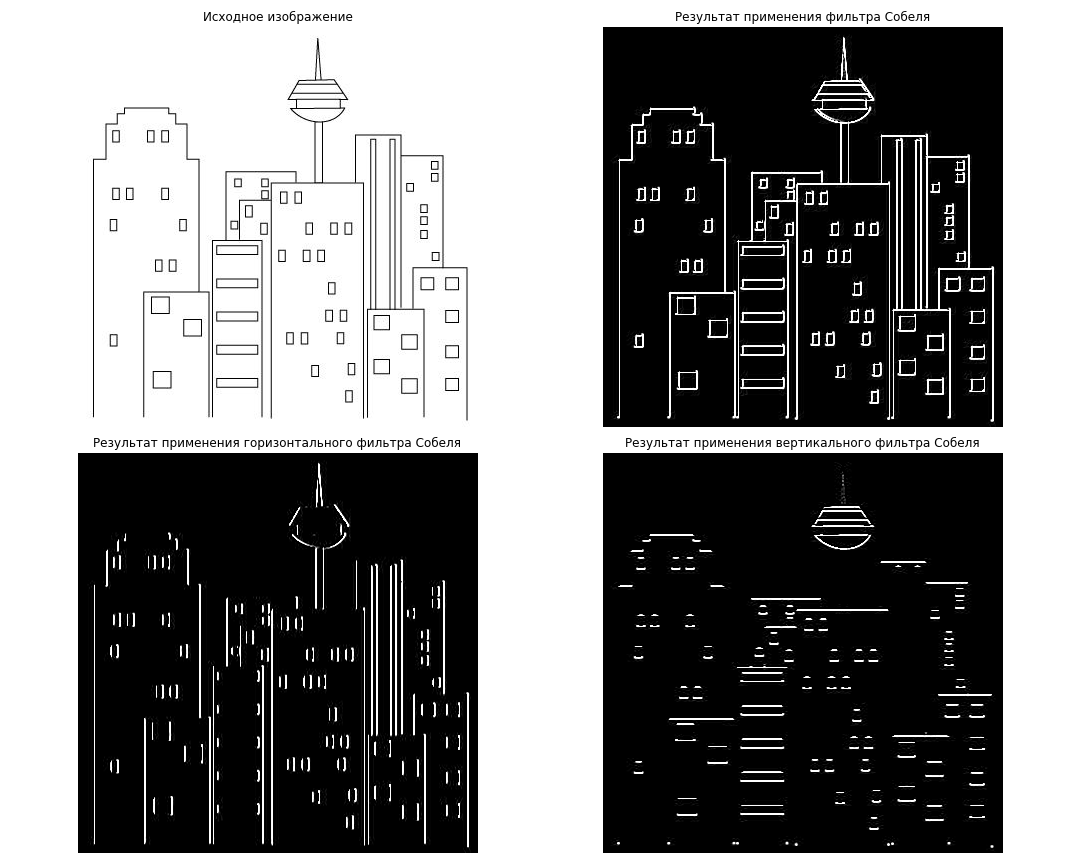
\includegraphics[width=\linewidth]{city_sobel}
	\caption{Применение оператора Собеля (1)}
\end{figure}

\begin{figure}[H]
	\centering
	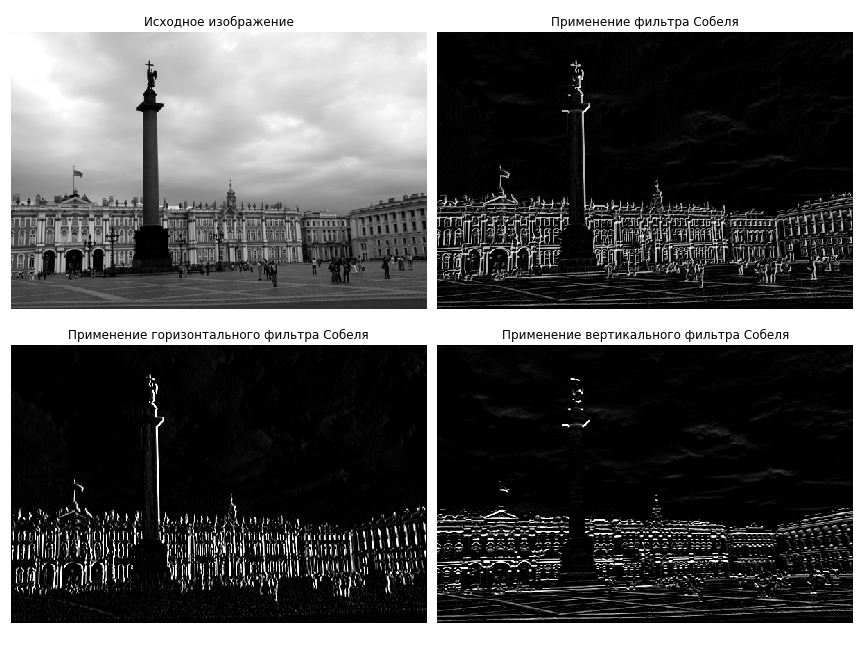
\includegraphics[width=\linewidth]{spb_sobel}
	\caption{Применение оператора Собеля (2)}
\end{figure}

\begin{figure}[H]
	\centering
	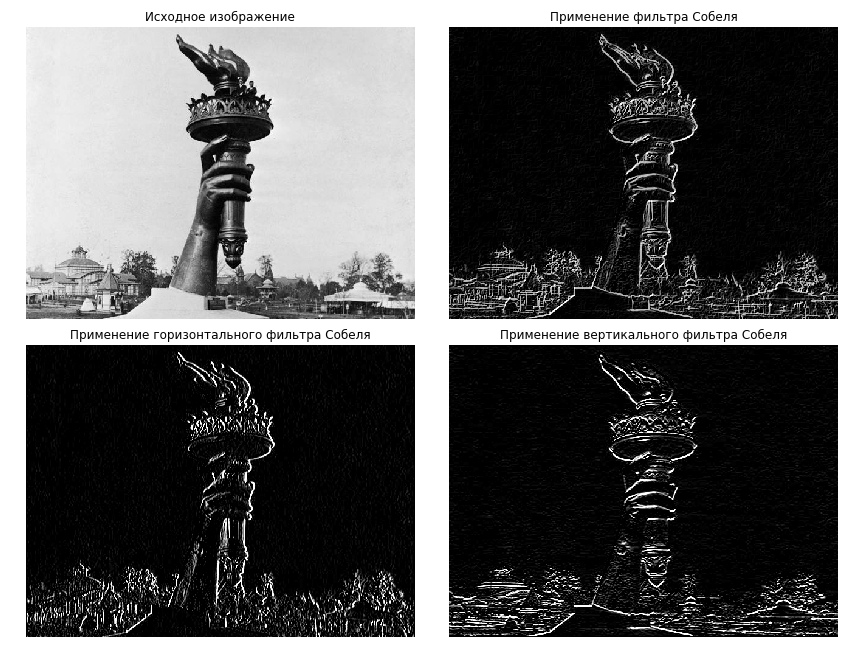
\includegraphics[width=\linewidth]{ny_sobel}
	\caption{Применение оператора Собеля (3)}
\end{figure}

\newpage

\section{Сравнение операторов}

Сравним результаты применения операторов к одному и тому же изображения. Для удобства выведем их рядом друг с другом.

\begin{figure}[H]
	\centering
	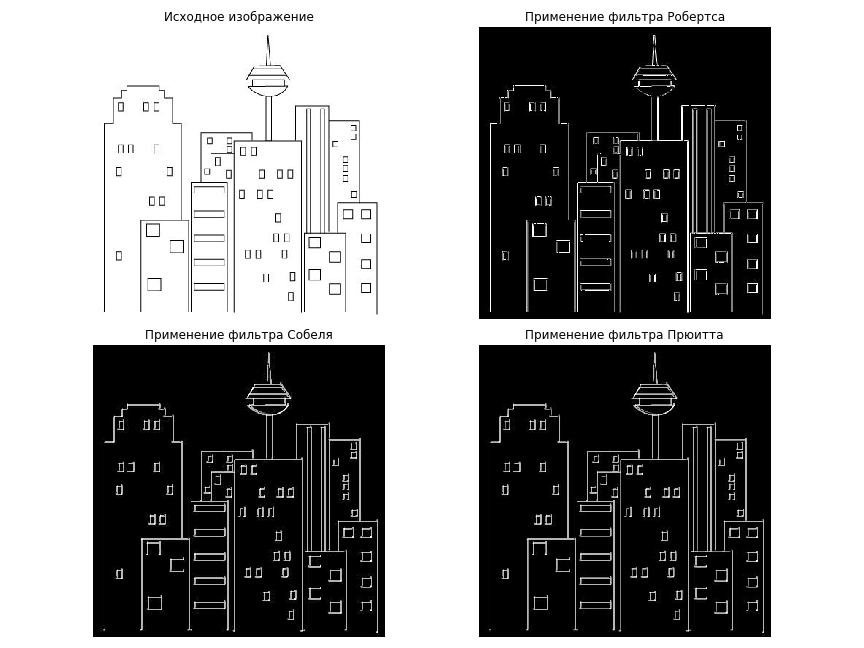
\includegraphics[width=\linewidth]{city_all}
	\caption{Применение всех операторов (1)}
\end{figure}

\begin{figure}[H]
	\centering
	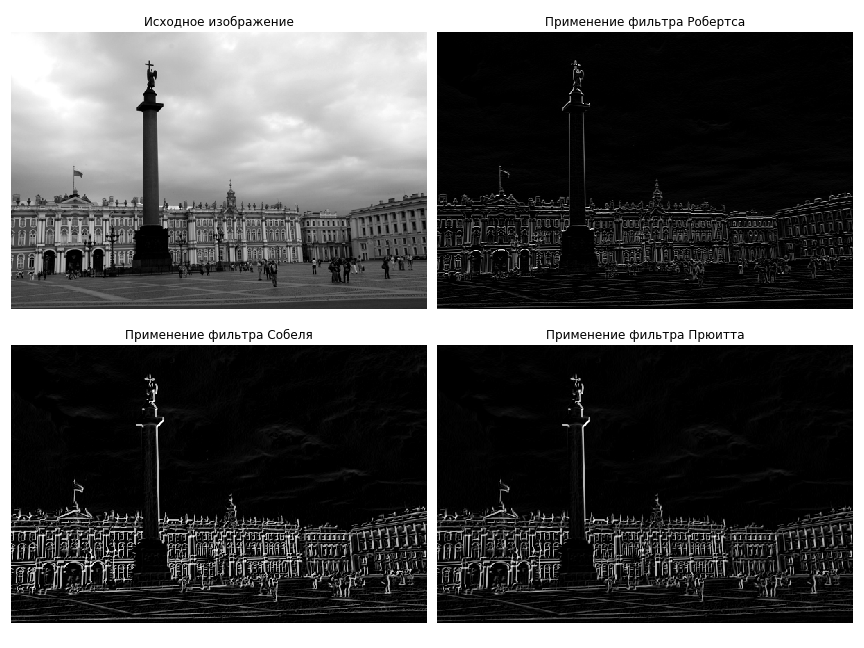
\includegraphics[width=\linewidth]{spb_all}
	\caption{Применение всех операторов (2)}
\end{figure}

\begin{figure}[H]
	\centering
	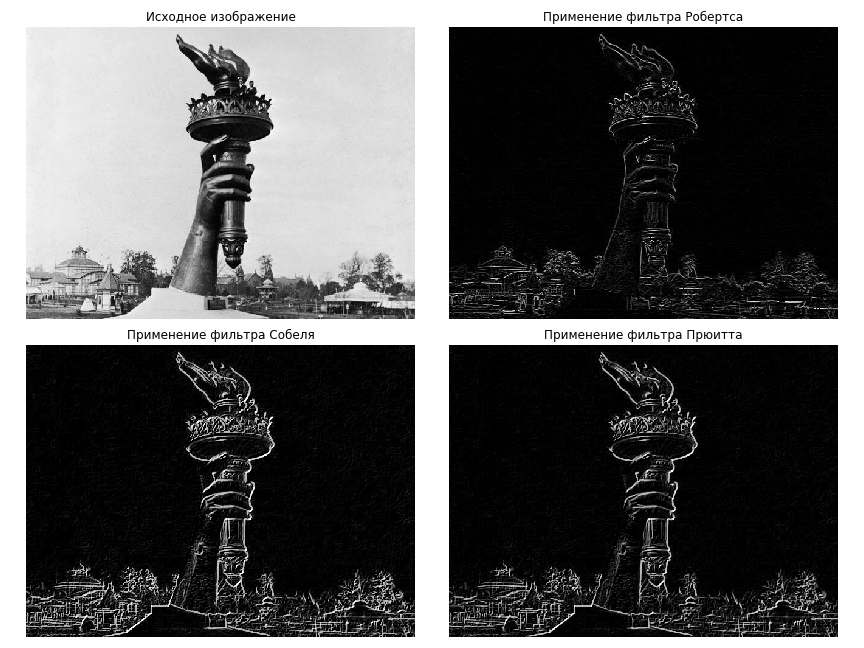
\includegraphics[width=\linewidth]{ny_all}
	\caption{Применение всех операторов (3)}
\end{figure}

\section{Выводы}

В данной работе были реализованы три оператора для детектирования границ на изображении:

\begin{itemize}
	\item оператор Робертса;
	\item оператор Собеля;
	\item оператор Прюитта.
\end{itemize}

Из получившихся изображений видно, что результаты применения операторов Собеля и Прюитта оказались очень схожи. Оба оператора высчитывают аппроксимацию горизонтально и вертикального градиента изображения, позволяя получить хорошую карту границ изображения. В то же время, оператор Робертса использует подход с поиском диагональных градиентов и работает хуже, упуская границы некоторых предметов на изображении.

\end{document}
